\documentclass[12pt]{report}

\usepackage[margin=0.7in]{geometry}
\usepackage{graphicx, verbatim, listings, fancyvrb, color, float, pdfpages}
\usepackage[english]{babel}
\usepackage[autostyle]{csquotes}
\usepackage{dirtree}
\usepackage{titling}
\usepackage{graphicx}
\usepackage{adjustbox}
\usepackage{amsmath}


\graphicspath{ {/Users/kim-anh/Documents/University/AIN/MDPPacman/report2/images/} }

\setlength{\droptitle}{-8em}   % This is your set screw

\title{6CCS3AIN Coursework: \\ Pacman in a hard(er) world}
\author{
  Kim-Anh Vu\\1707295\\
  \texttt{kim-anh.vu@kcl.ac.uk}
}
\date{November 2019}


\begin{document}
% Title page %
  \begin{titlepage}
    \maketitle
  \end{titlepage}
  \section*{Introduction}
    By implementing the MDP-solver and discovering the optimum values to set specific
    variables, the task was to be able to guide Pacman safely around the grid and
    win the game by consuming all of the food that is available.
    \vspace{-5mm}
    \section*{Implementation}
      The local variables are created when the MDPAgent has been initialised, which includes the initial number of food available in the game (which will contribute to creating a scale to increase the food reward as they become scarce), the width, height and walls of the layout. These are variables that will be used throughout the class.
      \newline \newline
      Firstly, to get the width and height of the layout, the corners list was used to find the maximum row and column value from the list of tuples and increment each value by 1. This is a better way of calculating the height and width than finding out which coordinates had the maximum y value and accessing the value directly using indexing, as the order of the coordinates could change, so height and width values would not be accurate.
      \newline \newline
      When the getAction() function in the MDPAgent class is called, the necessary information (current position, food, ghosts, legal, capsules) are assigned to local variables from the API provided.
      \newline \newline
      Then, two different multipliers are created. One that will be applied to food and capsules and the other will be applied to ghosts and positions around the ghosts. The reason behind scaling the ghost rewards consists of the fact that the pacman will see the negative reward as insignificant if the food reward is too high, therefore will be willing to kill itself. Both will use the proportion of food that is left out of the initial number of food, however the food multiplier is higher as the food reward is less positive than the ghost reward is negative.
      \newline \newline
      Then, a separate Board class is created, which width, height and the reward value for non-terminal states (which will be the default reward value for each position on the board) is passed to. This allows the setting of rewards of positions of the food, ghosts and capsules - replicating the layout of the board used. Also, rewards of potential positions the ghost can occupy in one or two moves (below) will have a value that is slightly more than the reward of ghosts, but much lower than the reward value for non-terminal states.
        \begin{figure}[H]
          \centering
          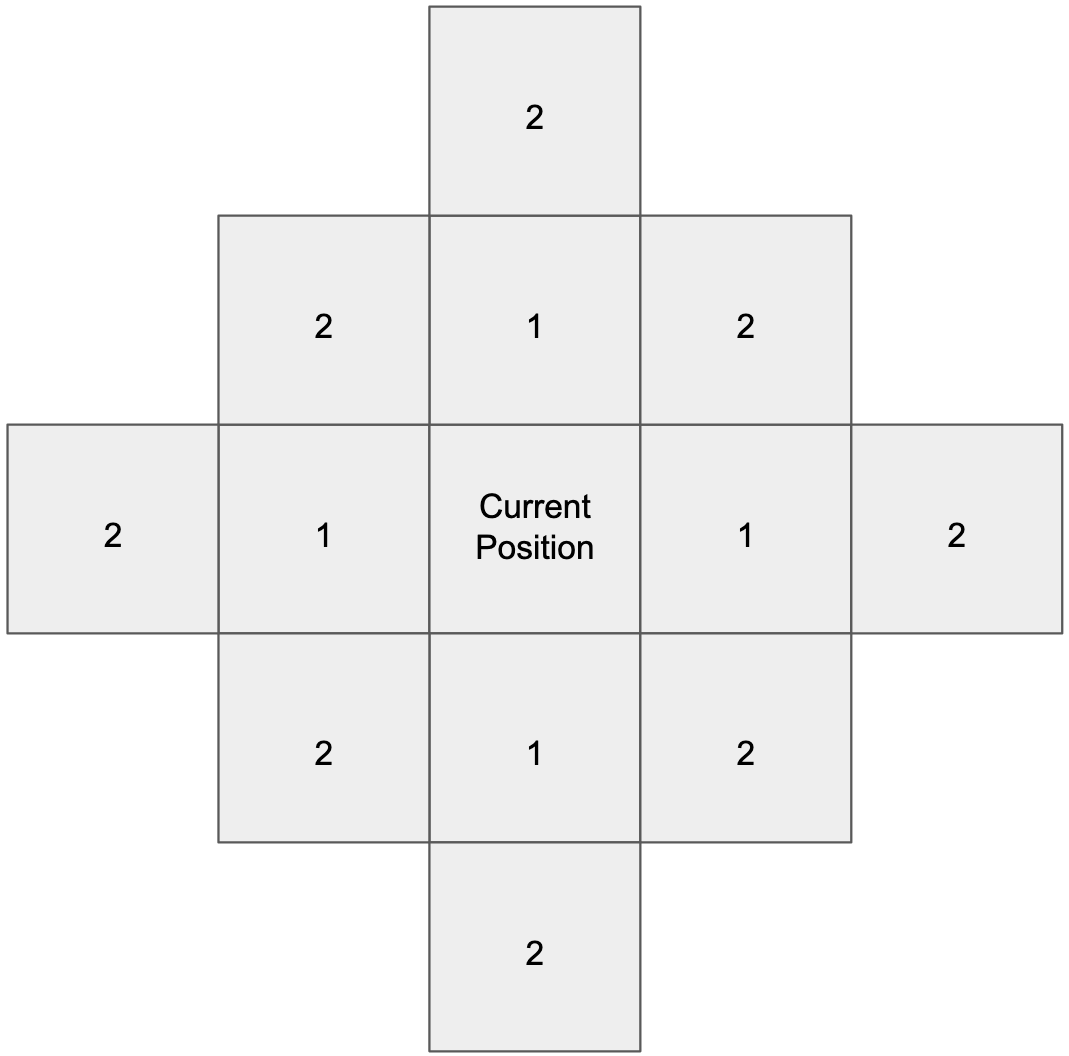
\includegraphics[scale=.25]{ghost_potential.png}
          \caption{Diagram showing potential positions ghost can make. Each square is marked by a number which represents move number of ghost.}
        \end{figure}
      \vspace{-5mm}
      \subsection*{Board Class}
        Public functions were created in the Board class to prevent other classes from accessing the board and its attributes directly, contributing to achieving loose coupling. Examples of functions that are in the Board class are setting values of each position or even taking in a list of positions and setting each position to the given value. Moreover, a function was created to convert the y coordinates, as the board (represented as a nested list) has row 0 as the top row, whereas the actual layout of the game's rows started from the bottom and the y coordinate increases as you go up. Therefore, you need a function that will be able to convert y coordinates of one board/layout to another.
        \newline \newline
        To obtain the updated board with each state containing an utility value, the function calls on the value iteration function.

      \subsection*{Value Iteration}
        `board' will be used to obtain the original rewards for each position.
        \newline `board\_copy' contains the deepcopy of the board that has been passed into the value iteration function and is the board that is used to update the utility for each state.
        \newline `U' is the previous state of `board\_copy'
        \newline
        \newline \hspace*{1cm} \underline{Example:}
        \newline \hspace*{1cm} You have updated the value at (x, y) in `board\_copy' and you needed the value at (x, y + 1) \hspace*{1cm} to do so. Now you need to update the value at (x, y + 1), which will need the old value of (x, \hspace*{1cm} y) which will be stored in `U'.
        \newline \newline
        This function iterates through `board\_copy' for a maximum of 14 times, resets the variable total\_difference (total difference between current board and future board as value iteration eventually converges) to zero and checks whether or not the cell is anything but a wall or a ghost. This is done by confirming if the position is not in `protected\_pos' which is a cocantenation of the list of ghost positions and list of wall positions. If the condition is satisfied `calculate\_expected\_utility' is invoked.
        \newline \newline
        `calculate\_expected\_utility' is a function that generates the potential next position of Pacman in a list called `coords'. All lists in this function's ordering is always the same, with the position or utility associated with going north always comes first, then east, south and finally west. The `coord' list which initially contains positions is looped through and any position that is a currently occupied by a wall is replaced with the current position. Due to this strategy, there is no need to check if the index is out of bounds. Then, pair each position with its corresponding reward/utility. The list is then looped through to find the positions that are at a right angle to each coordinate.

        \begin{figure}[H]
          \centering
          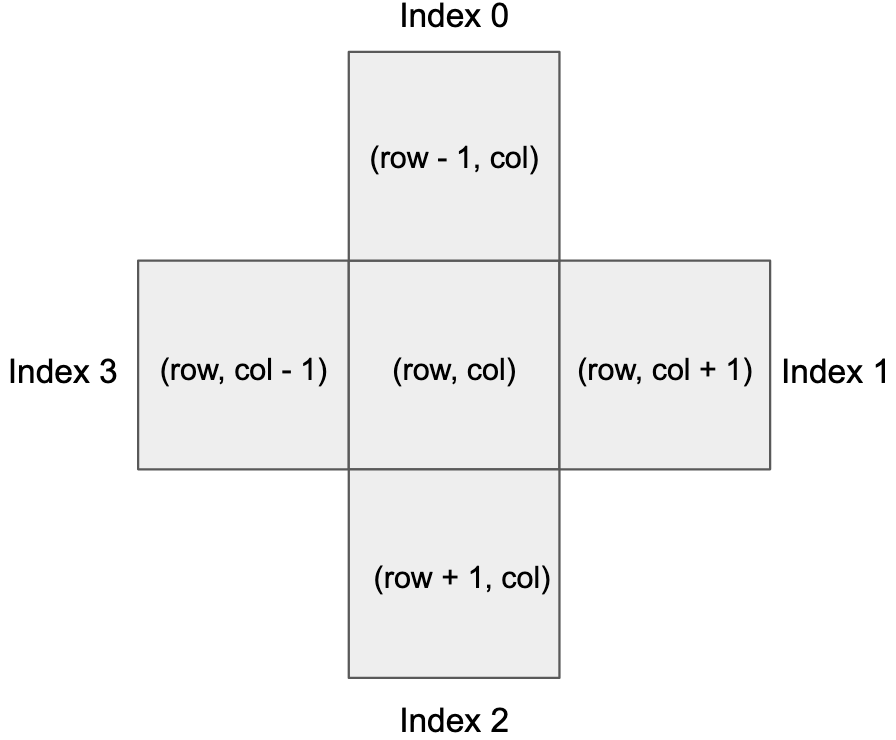
\includegraphics[scale=.47]{calculate_utility_diagram.png}
        \end{figure}
        \begin{table}[H]
          \begin{center}
            \begin{tabular}{c|c|c}
              \textbf{Intended Action} & \textbf{90$^{\circ}$ Anti-Clockwise Action} & \textbf{90$^{\circ}$ Clockwise Action}\\
              \hline
              North (index 0) & West (index 3) & East (index 1)\\
              East (index 1) & North (index 0) & South (index 2)\\
              South (index 2) & East (index 1) & West (index 3)\\
              West (index 3) & South (index 2) & North (index 0)\\
            \end{tabular}
            \caption{Possible actions undertaken due to probability depending on intended action.}
            \label{tab:table1}
          \end{center}
        \end{table}
        \vspace{-5mm}
        From looking at the diagram and the table, you can now work out any possible action from an intended action using indices and modular arithmetic - this removes the need to create many if statements. To get the index of the position which is 90$^{\circ}$ anti-clockwise to the intended action, you need to add 3 to the corresponding index to your action, mod 4 and to get the position which 90$^{\circ}$ clockwise to the intended action, you need to add 1 to the corresponding index to your action, mod 4.
        \newline \newline
        Now that you know all coordinates that are associated when making a certain move, you multiply the value of the position that you will end up when making the intended action by 0.8 and the value of the positions if you make an action 90$^{\circ}$ to the intended action by 0.1. After, place the sum of the values in a tuple with the intended action and add it to the `prob' list. When calculations are done for all possible actions, return the `prob' list.
        \newline \newline
        The `value\_iteration' only takes the first element of each tuple in the list returned by `calculate\_expected \_utility', which is the expected utility for each intended action. The maximum expected utility is calculated and this value is inputted in the Bellman's equation, in which the answer is then assigned as the utility of that position on the board.
        \newline \newline
        In this case, value iteration will inevitably converge due to factors like the state and action space are finite and although the environment is continuous, the discount factor is less than 1 (0.9). However, convergence can take a long time, therefore a threshold is introduced to break the loop, hence reducing the running time, at a point where a long running time is not an acceptable trade-off for further iterations - slightly improving the accuracy of the policy.
        \newline \newline
        The total difference between the previous board and the new board in terms of utilities is calculated at the end of each iteration and if the total is less than the threshold, then the difference is so small that iterating through the board again is obsolete, therefore we break. However, if the total difference between the two boards is larger than the threshold, then we depreciate the variable `iterations' by 1 and loop through the new board. When `iterations' is equal to zero or when we break from the loop, the new board calculated is returned to `getAction', where `getAction' then calls on `calculate\_expected\_utility' with the current position of the pacman and the new board obtained from `value\_iteration' as parameters. The list returned is filtered to only include actions that are legal and then returns `makeMove' with the action with the maximum expected utility as the parameter.

        The code was tested to return `makeMove' with the action with the maximum expected utility without filtering actions that are not present in the `api.legalActions' beforehand. The results were very poor (further elaborated in `Performance Analysis'), thus the decision to filter the list first, before finding the maximum expected utility was made.

      \section*{Creativity}
        \begin{itemize}
          \item Identifying positions that are at a right angle to the current position by manipulating indicies using modular arithmetic. This avoids the need to have many if statements for every action. In `calculate\_expected\_utility, only one if statement was used.
          \item Setting the reward of the positions that surround the ghosts to a value that is larger than the ghost reward but less than the non-terminal reward. This is essentially a warning to the pacman that going in that direction means they will be closer to the ghost.
          \item Used threshold and a limit to how many iterations you have to loop through the board. Prevents value\_iteration from running infinitely and if the difference is small enough, does not waste computational power and time to iterate again.
          \item Scaled food reward, so as there is less food available, the reward of the food increases. This encourages pacman to move towards the scarce food, rather than just wander around and happen to be at a closer distance to food. This is achieved by using two separate multipliers - one for ghost-related rewards and the other is food-related rewards.
          \vspace{-2mm}
            \begin{align*}
              food\_multiplier &= 0.8 \left(\frac{current\_num\_food}{initial\_num\_of\_food}\right)^2 + 6
            \end{align*}
            \vspace{-5mm}
            \begin{align*}
              ghost\_multiplier &= 0.2 \left(\frac{current\_num\_food}{initial\_num\_of\_food}\right)^2 + 3
            \end{align*}
          \item Carried out a paired t-test and the two-tailed P value for smallGrid and mediumClassic is less than 0.0001, thus the difference is considered to statistically significant.
        \end{itemize}

      \section*{Performance Analysis}
      \subsection*{Base Performance}
      These are the results that was noted at the start of the coursework. The base results will be developed upon.
        \begin{table}[H]
          \begin{center}
            \begin{adjustbox}{max width=\textwidth}
            \begin{tabular}{*{3}{c}}

              \textbf{} & \textbf{Win Rate (\%)} & \textbf{Time Taken (s)}\\
              \hline
                    Small Grid & 36 & 2.88 \\
                    Medium Classic & 23 & 131.17 \\

            \end{tabular}
            \end{adjustbox}
            \caption{For each iteration, the game was run 100 times, threshold = 0.4, ghost reward = -1, non-terminal reward = -0.04, food reward = 1, capsule reward = 1, number of iterations = 6.}
            \label{tab:table4}
          \end{center}
        \end{table}
        \vspace{-5mm}
        \subsection*{Number of Iterations}
          \begin{table}[H]
            \begin{center}
              \begin{adjustbox}{max width=\textwidth}
              \begin{tabular}{*{5}{c}}
                \textbf{No. of Iterations} & \textbf{Small Grid Win Rate (\%)} & \textbf{Time Taken(s)} & \textbf{Medium Classic Win Rate (\%)} & \textbf{Time Taken (s)}\\
                \hline
                7 & 52 & 6.25 & 26 & 445.25\\
                8 & 63 & 7.42  & 30 & 759.76\\
                9 & 53 & 12.32  & 35 & 1110.07\\
                10 & 60 & 16.22 & 41 & 1228.42\\
                11 & 70 & 26.10 & 40 & 1660.70\\
                12 & 63 & 30.46 & 37 & 2045.95\\
                13 & 58 & 36.31 & 41 & 2200.12\\
                14 & 64 & 46.89 & 44 & 2376.07\\
                15 & 64 & 66.31 & 43 & 2495.31\\
                16 & 59 & 50.44 & 38 & 2412.19\\
                17 & 59 & 58.29 & 40 & 2499.86\\
                18 & 69 & 68.32 & 42 & 2503.80\\
                19 & 60 & 85.30 & 39 & 2366.64\\
                20 & 56 & 64.38 & 38 & 1544.07\\
              \end{tabular}
              \end{adjustbox}
              \caption{Finding optimum number of iterations that results in highest win rate. For each iteration, the game was run 100 times, $\gamma$ = 0.9, ghost reward = -3, non-terminal reward = -0.04, food reward = 1, capsule reward = 2.}
              \label{tab:table2}
            \end{center}
          \end{table}
          \vspace{-13mm}
        \begin{figure}[H]
          \centering
            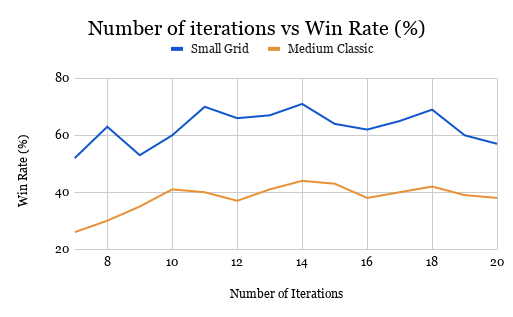
\includegraphics[scale=.6]{iterations_graph.png}
            \caption{Graph showing relationship between number of iterations and win rate for each layout}
        \end{figure}
          Starting point for number of iterations was initially 1, however the average win rate for mediumClassic was 14\% and after leaving smallGrid to run for an hour, the first game was still ongoing. Therefore, it was realised that the starting point needs to be considerably higher, thus 7 was randomly chosen as the official starting point. It was observed that as the number of iterations positively diverged from 7, the higher the win rate for both layouts. However, as it reaches 14 for both layouts, the win rate plateaus. There are fluctuations in win rate from 14 onwards, but it may be due to the non-deterministic nature of the game, therefore the optimal iteration value chosen was 14.

      \subsection*{Threshold}
        \begin{table}[H]
          \begin{center}
            \begin{adjustbox}{max width=\textwidth}
            \begin{tabular}{*{5}{c}}
              \textbf{Threshold} & \textbf{Small Grid Win Rate (\%)} & \textbf{Time Taken(s)} & \textbf{Medium Classic Win Rate (\%)} & \textbf{Time Taken (s)}\\
              \hline
              0.1 & 64 & 125.85 & 48 & 7057.32\\
              0.2 & 65 & 110.23 & 33 & 7011.25\\
              0.3 & 62 & 98.34 & 39 & 6843.77\\
              0.4 & 60 & 72.67 & 40 & 6305.70\\
              0.5 & 62 & 54.66 & 42 & 6506.80\\
              0.6 & 58 & 42.23 & 34 & 3479.87\\
              0.7 & 61 & 46.75 & 39 & 3134.97\\
              0.8 & 56 & 30.63 & 31 & 2423.78\\
              0.9 & 61 & 28.95 & 37 & 2664.63\\
              1.0 & 61 & 25.10.66 & 39 & 2709.44\\
            \end{tabular}
            \end{adjustbox}
            \caption{Finding optimum threshold that results in highest win rate. For each iteration, the game was run 100 times, $\gamma$ = 0.9, ghost reward = -3, non-terminal reward = -0.04, food reward = 1, capsule reward = 2, range = (0.1, 1.0)}
            \label{tab:table3}
          \end{center}
        \end{table}
        \vspace{-13mm}
        \begin{figure}[H]
          \centering
          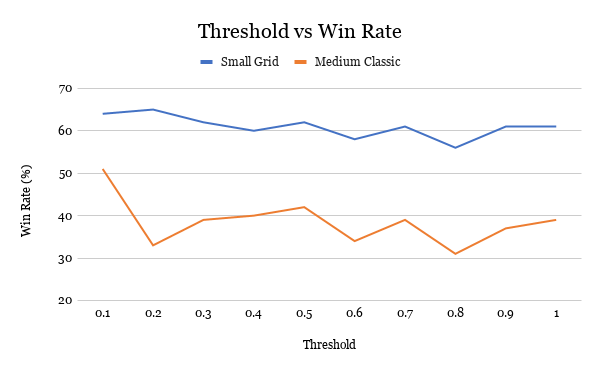
\includegraphics[scale=.6]{threshold_graph.png}
          \caption{Graph showing relationship between threshold and win rate for each layout}
        \end{figure}

          The table shows the optimum for smallGrid is between 0.1 and 0.2 and the optimum for mediumClassic is 0.1. Furthermore, if you are to compare the results between using a fixed number of iterations (14) and a threshold (0.1), you can see the results for smallGrid are similar, however for mediumClassic, using a threshold slightly outperforms using a fixed number iterations alone. On the contrary, the running time difference between using threshold alone and using a fixed number of iterations is significant as on average it takes many more iterations to have a total difference that is less than 0.1. Due to evaluating the advantages and disadvantages of using different iterating strategies, it was decided to use mainly a fixed number of iterations as the win rate would be similar to using a threshold of 0.1, taking 46.81s on average faster for each game. Although, a threshold is implemented as well, so if there is an instance where the total difference is less than threshold and the program has ran less than 14 iterations, it will break the loop which reduces overall running time and computational power.

      \subsection*{Discount Factor}
        \begin{table}[H]
          \begin{center}
            \begin{adjustbox}{max width=\textwidth}
              \begin{tabular}{*{5}{c}}

                \textbf{Discount Factor} & \textbf{Small Grid Win Rate (\%)} & \textbf{Time Taken(s)} & \textbf{Medium Classic Win Rate (\%)} & \textbf{Time Taken (s)}\\
                \hline
                0.0 & 6 & 1.28 & 0 & 48.19\\
                0.1 & 1 & 1.75 & 0 & 129.14\\
                0.2 & 5 & 1.62 & 14 & 181.35\\
                0.3 & 7 & 2.41 & 17 & 233.43\\
                0.4 & 12 & 3.31 & 31 & 406.39\\
                0.5 & 64 & 5.06 & 34 & 511.38\\
                0.6 & 66 & 6.62 & 35 & 504.32\\
                0.7 & 69 & 9.44 & 43 & 626.83\\
                0.8 & 66 & 9.47 & 46 & 572.78\\
                0.9 & 75 & 9.52 & 49 & 511.64\\
                1.0 & 59 & 9.25 & 37 & 484.08\\
              \end{tabular}
            \end{adjustbox}
            \caption{Finding optimum discount factor that results in highest win rate. For each iteration, the game was run 100 times, threshold = 0.1, ghost reward = -3, non-terminal reward = -0.04, food reward = 1, capsule reward = 2. Number of iterations = 14.}
              \label{tab:table4}
        \end{center}
      \end{table}
      \vspace{-13mm}
      \begin{figure}[H]
        \centering
        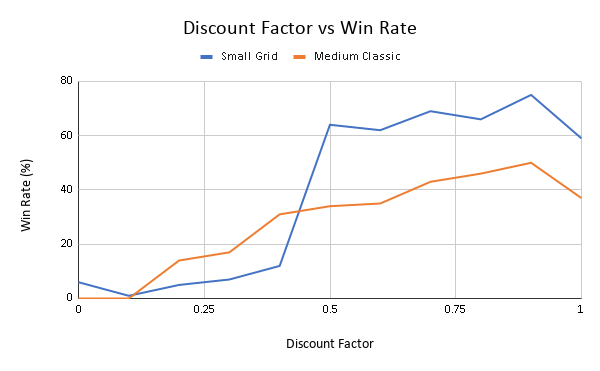
\includegraphics[scale=.6]{discountfactor_graph.png}
        \caption{Graph showing relationship between discount factor and win rate for each layout}
      \end{figure}
      There is a common trend for both layouts where win rate increases from 0.0 to 0.9, however when the discount factor is 1.0, the win rate for both layouts dips drastically (21.3\% and 26\% decrease for smallGrid and mediumClassic respectively).

      \subsection*{Surrounding Ghosts Reward}
      This is to test the win rate of each layout when adding a more negative reward to positions the ghosts can occupy in two moves.
        \begin{table}[H]
          \begin{center}
            \begin{adjustbox}{max width=\textwidth}
            \begin{tabular}{*{3}{c}}
              \textbf{} & \textbf{Win Rate (\%)} & \textbf{Time Taken(s)} \\
              \hline
                    Small Grid & 78 & 11.98 \\
                    Medium Classic & 62 & 15.27 \\

            \end{tabular}
            \end{adjustbox}
            \caption{For each iteration, the game was run 100 times, threshold = 0.1, ghost reward = -5, non-terminal reward = -0.04, food reward = 1, capsule reward = 2, number of iterations = 14.}
            \label{tab:table4}
          \end{center}
        \end{table}
        \vspace{-9mm}
        The results are significantly higher due to the pacman planning its move, taking into account the possible ghosts' positions 2 moves ahead - decreasing vulnerability and increasing chances of survival.

      \subsection*{Reward}
        \begin{table}[H]
          \begin{center}
            \begin{adjustbox}{max width=\textwidth}
              \begin{tabular}{*{5}{c}}

                \textbf{Reward} & \textbf{Small Grid Win Rate (\%)} & \textbf{Time Taken(s)} & \textbf{Medium Classic Win Rate (\%)} & \textbf{Time Taken (s)}\\
                \hline
                -2 & 63 & 11.04 & 34 & 4458.40\\
                -3 & 64 & 11.29 & 36 & 4564.48\\
                -4 & 63 & 59.60 & 31 & 4935.20\\
                -5 & 61 & 59.51 & 44 & 5247.78\\
                -6 & 70 & 66.72 & 36 & 4914.50\\
                -7 & 72 & 94.30 & 46 & 5175.68\\
                -8 & 71 & 117.11 & 43 & 4698.51\\
                -9 & 69 & 118.53 & 41 & 3857.05\\
                -10 & 70 & 132.62 & 42 & 2564.55\\
                -11 & 72 & 146.82 & 39 & 2168.11\\
                -12 & 69 & 61.70 & 40 & 1691.51\\
              \end{tabular}
            \end{adjustbox}
            \caption{Finding optimum reward ratio that results in highest win rate. For each iteration, the game was run 100 times, threshold = 0.1, non-terminal reward = -0.04, food reward = 1, capsule reward = 2, number of iterations = 14. Every reward was constant except from the ghost reward and the reward of the positions surrounding the ghosts. Difference between reward of the positions surrounding the ghosts and reward of ghosts is 1, where ghosts is always more negative.}
              \label{tab:table4}
        \end{center}
      \end{table}
      \vspace{-12mm}
      \begin{figure}[H]
        \centering
        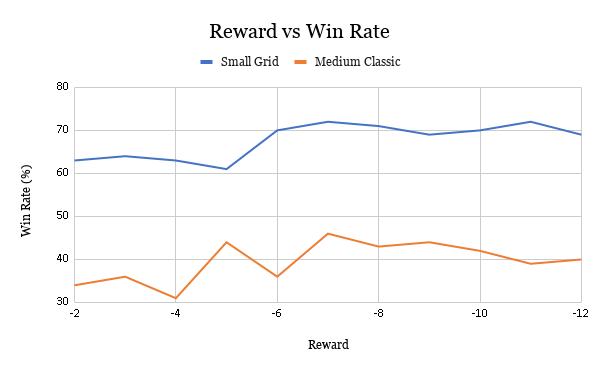
\includegraphics[scale=.6]{reward_graph.png}
        \caption{Graph showing relationship between changing the ghost-related rewards and win rate for each layout}
      \end{figure}
      For both layouts, win rate increases as you negatively diverge from a reward of -2 until you reach -6 which is when it plataeus. Thus, -7 and -6 was chosen to be the ghost reward and surround positions around the ghost reward respectively, to be comfortable in the optimum range.

      \subsection*{makeMove}
      Testing to decide whether or not to call makeMove on the action that has the maximum utility out of the four possible actions or on the action that has the maximum utility out of all legal actions.
        \begin{table}[H]
          \begin{center}
            \begin{adjustbox}{max width=\textwidth}
            \begin{tabular}{*{5}{c}}
              \textbf{} & \textbf{Small Grid Win Rate (\%)} & \textbf{Time Taken(s)} & \textbf{Medium Classic Win Rate (\%)} & \textbf{Time Taken (s)}\\
              \hline
                    Filtered & 75 & 1.28 & 40 & 1016.87\\
                    Unfiltered & 0 & 6.79 & 0 & 707.20\\
            \end{tabular}
            \end{adjustbox}
            \caption{For each iteration, the game was run 100 times, threshold = 0.1, ghost reward = -5, non-terminal reward = -0.04, food reward = 1, capsule reward = 2, number of iterations = 14.}
            \label{tab:table4}
          \end{center}
        \end{table}
        \vspace{-9mm}
        Unfiltered consists of potentially returning Directions.STOP, which reduces the win rate to 0 every time for each layout, potentially due to the fact that it gives the ghosts more time to catch up with the pacman, increasing the pacman's vulnerability and chance of death. Thus, the decision was made to find the maximum utility of an action only if it is legal.

        \subsection*{Ghost Reward Change Due To Consumption of Capsule}
          \begin{table}[H]
            \begin{center}
              \begin{adjustbox}{max width=\textwidth}
              \begin{tabular}{*{5}{c}}

                \textbf{} & \textbf{Small Grid Win Rate (\%)} & \textbf{Time Taken(s)} & \textbf{Medium Classic Win Rate (\%)} & \textbf{Time Taken (s)}\\
                \hline
                      No Change in Reward & 59 & 14.90 & 40 & 775.35\\
                      Constant Reward & 62 & 15.27 & 42 & 777.20\\

              \end{tabular}
              \end{adjustbox}
              \caption{For each iteration, the game was run 100 times, threshold = 0.1, ghost reward = -5, non-terminal reward = -0.04, food reward = 1, capsule reward = 2, number of iterations = 14.}
              \label{tab:table4}
            \end{center}
          \end{table}
          \vspace{-9mm}
          The choice to keep the ghosts' rewards constant throughout the game was made due to the fact that it takes roughly the same time to run both layouts and win rates are similar. There was a drastic difference in win rate when you only changed ghost-related rewards when the scared time of the ghost was $<$4 - this may be because the pacman can become much more closer to the ghost due to its invincibility, but when the ghosts are not scared anymore, the pacman will not have time to distance itself away from the ghosts, thus they are much more vulnerable to dying. Win rate significantly improves when you change the ghost-related rewards back at 4s or more, as there is more time for pacman to escape from the vicinity of the ghosts.

            \subsection*{Scaling Food Reward}
            Due to its parabolic feature (y moves in a positive direction as you increase x slowly at first and then much faster as x is larger), the multiplier will be represented as a quadratic equation. This further encourages pacman to move towards the scarce food as the game progresses.
              \begin{table}[H]
                \begin{center}
                  \begin{adjustbox}{max width=\textwidth}
                    \begin{tabular}{*{5}{c}}
                      \textbf{Food Coefficient} & \textbf{Small Grid Win Rate (\%)} & \textbf{Time Taken(s)} & \textbf{Medium Classic Win Rate (\%)} & \textbf{Time Taken (s)}\\
                    \hline
                          0.3 & 13 & 7.97 & 0 & 937.54 \\
                          0.4 & 25 & 10.01 & 2 & 992.37 \\
                          0.5 & 30 & 20.18 & 3 & 975.97 \\
                          0.6 & 36 & 19.32 & 6 & 985.01 \\
                          0.7 & 37 & 32.51 & 37 & 32.51 \\
                          0.8 & 49 & 31.57 & 41 & 35.76 \\
                          0.9 & 41 & 10.93 & 32 & 45.32 \\
                          1.0 & 38 & 18.88 & 13 & 524.53 \\
                          1.5 & 36 & 15.63 & 16 & 532.67 \\
                          2.0 & 36 & 10.97 & 5 & 560.82 \\

                  \end{tabular}
                  \end{adjustbox}
                  \caption{For each iteration, the game was run 100 times, threshold = 0.1, ghost reward = -7, non-terminal reward = -0.04, food reward = 1, capsule reward = 2, number of iterations = 14. Random coefficient of 0.2 was given to the ghost multiplier.}
                  \label{tab:table4}
                \end{center}
              \end{table}
              \vspace{-9mm}
              \begin{table}[H]
                \begin{center}
                  \begin{adjustbox}{max width=\textwidth}
                    \begin{tabular}{*{5}{c}}
                      \textbf{Food Constant} & \textbf{Small Grid Win Rate (\%)} & \textbf{Time Taken(s)} & \textbf{Medium Classic Win Rate (\%)} & \textbf{Time Taken (s)}\\
                    \hline
                          1 & 41 & 11.74 & 0 & 937.54 \\
                          2 & 47 & 11.15 & 2 & 992.37 \\
                          3 & 47 & 19.18 & 3 & 975.97 \\
                          4 & 44 & 19.32 & 6 & 985.01 \\
                          5 & 44 & 42.79 & 23 & 2056.38 \\
                          6 & 45 & 57.25 & 35 & 2556.24 \\
                          7 & 41 & 10.93 & 29 & 2565.98 \\
                          8 & 38 & 18.88 & 24 & 2783.43 \\
                          9 & 36 & 15.63 & 27 & 2713.70 \\
                          10 & 37 & 56.23 & 28 & 2448.00 \\

                  \end{tabular}
                  \end{adjustbox}
                  \caption{For each iteration, the game was run 100 times, threshold = 0.1, ghost reward = -7, non-terminal reward = -0.04, food reward = 1, capsule reward = 2, number of iterations = 14, ghost multiplier coefficient = 0.2, food multiplier coefficient = 0.8.}
                  \label{tab:table4}
                \end{center}
              \end{table}

              \vspace{-9mm}
              \begin{table}[H]
                \begin{center}
                  \begin{adjustbox}{max width=\textwidth}
                    \begin{tabular}{*{5}{c}}
                      \textbf{Ghost Constant} & \textbf{Small Grid Win Rate (\%)} & \textbf{Time Taken(s)} & \textbf{Medium Classic Win Rate (\%)} & \textbf{Time Taken (s)}\\
                    \hline
                          1 & 64 & 12.68 & 46 & 1479.54 \\
                          2 & 75 & 24.10 & 45 & 992.37 \\
                          3 & 81 & 25.31 & 54 & 975.97 \\
                          4 & 79 & 36.68 & 51 & 2811.19 \\
                          5 & 78 & 42.79 & 45 & 1002.45 \\
                          6 & 71 & 57.25 & 42 & 954.56\\
                          7 & 75 & 60.18 & 41 & 843.98\\
                          8 & 80 & 83.61 & 50 & 1741.97 \\
                          9 & 73 & 68.10 & 58 & 861.74 \\
                          10 & 70 & 71.12 & 5 & 560.82 \\

                  \end{tabular}
                  \end{adjustbox}
                  \caption{For each iteration, the game was run 100 times, threshold = 0.1, ghost reward = -7, non-terminal reward = -0.04, food reward = 1, capsule reward = 2, number of iterations = 14, ghost multiplier coefficient = 0.2, food multiplier coefficient = 0.8, food constant = 6}
                  \label{tab:table4}
                \end{center}
              \end{table}
                \vspace{-9mm}
              \hspace{-8mm} From the tests, it can be concluded that for the food multiplier, the optimal coefficient is 0.8 and optimal constant is 6. Furthermore, for the ghost multiplier, the coefficient is 0.2 and optimal constant would be 3 as after 3, the results are quite similar. Fluctuations are most likely be due to the stochastic environment.
  \section*{Optimised Performance}
  Taking into account the findings from testing. The optimised MDP agent has been created by combining all optimal values observed from testing.

  \begin{table}[H]
    \begin{center}
      \begin{adjustbox}{max width=\textwidth}
      \begin{tabular}{*{3}{c}}
        \textbf{} & \textbf{Small Grid Win Rate (\%)} & \textbf{Medium Classic Win Rate (\%)} \\
        \hline
              Base & 36 & 23 \\
              Optimal & 79 & 53 \\

      \end{tabular}
      \end{adjustbox}
    \end{center}
  \end{table}
  \vspace{-9mm}
  The two-tailed P value for smallGrid and mediumClassic is less than 0.0001, thus the difference is considered to statistically significant.

\end{document}
